% Methodology section

\subsection{Opetopes}
Originally developed by Baez and Dolan \citep{baez1997higher}, opetopes are mathematical objects that were introduced to weak n-Categories. They are higher-dimensional generalizations of simplicial complexes, capturing directed higher-order interactions with explicit compositional structure. There are multiple ways to define opetopes, but the most common approach is to define them recursively by their boundaries, which are themselves opetopes of lower dimensions. A more traditional way is to define opetopes is using another algebraic structure called operads, which are used to model algebraic structures with multiple operations. Opetopes are a generalization of operads, and they can be used to model higher-dimensional structures with multiple operations. Hence opetopes comes from the word "operation" and "polytope".

We will first look at the more traditional definition of opetopes using operads, and then we will look at the more modern definition of opetopes using boundaries.

\subsubsection{Operads}

Operads are algebraic structures that generalize monoids, groups, and other algebraic structures. Operads consists of:

\begin{itemize}
  \item A collection of operations of different arities.
  \item A notion of composition of these operations.
  \item The composition operations obey certain conditions - associativity and unitality.
\end{itemize}

\subsubsection{Operads: Formal Definition}

Consider a set $\mathbb{X}$, and an integer $n \in \mathbb{N}$.

Now consider a set of functions, lets call it $\mathbb{P}$, where each function $f$ has the signature $\mathbb{X}^n \to \mathbb{X}$:

\begin{equation}
  \mathbb{P}(n) = \{f: \mathbb{X}^n \to \mathbb{X}\}
\end{equation}

where $\mathbb{X}^n$ is the cartesian product of $\mathbb{X}$ with itself $n$ times, i.e.

\begin{equation}
  \mathbb{X}^n = \mathbb{X} \times \mathbb{X} \times \ldots \times \mathbb{X}
\end{equation}

i.e. all of these functions $f$ take in $n$ arguments from $\mathbb{X}$ and return a single element from $\mathbb{X}$.

\begin{figure}[h]
\centering
    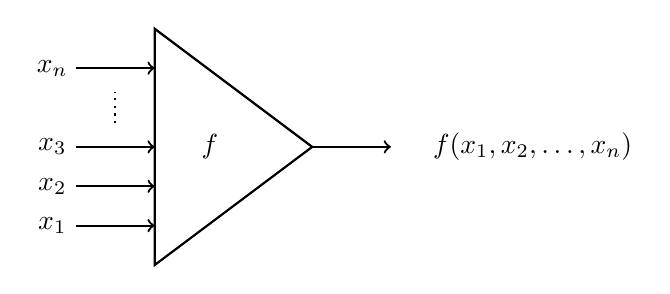
\begin{tikzpicture}
        % Draw the triangle with vertical left edge
        \draw[thick, fill=white] (0,0) -- (0,3) -- (2,1.5) -- cycle;

        % Draw input arrows
        \draw[->, thick] (-1,0.5) -- (0,0.5);
        \draw[->, thick] (-1,1) -- (0,1);
        \draw[->, thick] (-1,1.5) -- (0,1.5);
        \draw[dotted, thick] (-0.5,1.8) -- (-0.5,2.2);
        \draw[->, thick] (-1,2.5) -- (0,2.5);

        % Draw output arrow
        \draw[->, thick] (2,1.5) -- (3,1.5);

        % Add labels
        \node at (0.7,1.5) {$f$};
        \node at (-1.3,0.5) {$x_1$};
        \node at (-1.3,1) {$x_2$};
        \node at (-1.3,1.5) {$x_3$};
        \node at (4.8,1.5) {$f(x_1,x_2,\ldots,x_n)$};
        \node at (-1.3,2.5) {$x_n$};
    \end{tikzpicture}
\end{figure}

If we have a bunch of these sets of functions $\mathbb{P}(k_i)$ for each $k_i \in \mathbb{N}$, then we can define a composition operation $\circ$ on these functions as follows:

Let $f_i \in \mathbb{P}(k_i)$ be a function that takes in $k_i$ arguments from $\mathbb{X}$ and returns a single element from $\mathbb{X}$.

\begin{equation}


